\documentclass[12pt, a4paper]{article}

\usepackage[hidelinks]{hyperref}
\usepackage[tmargin=1in, bmargin=1in]{geometry}
\usepackage{parskip}
\usepackage{amssymb}
\usepackage{amsmath}
\usepackage[shortlabels]{enumitem}
\usepackage[dutch]{babel}
\selectlanguage{dutch}
\usepackage{pgfplots}
\pgfplotsset{width=7.5cm, compat=1.18}
\usepackage{amsthm}

\begin{document}

\title{Lineare Algebra - Inleveropgave 1}
\author{Brechtje Poppen - Lotte Gritter - Boris van Boxtel}
\date{23 september 2022 - Week 38} 

\maketitle
\pagenumbering{gobble}

\begin{enumerate}[(a).]
    \item \label{opdrachta}
    Stel $z^n = 1$ met $z \in \mathbb{C}$ en $n \in \mathbb{N}$. Dan is $z$ te schrijven als volgt: $z = re^{i\phi}$, dus $z^n = r^ne^{in\phi} = 1$.

    Omdat $w_1 = w_2$ met $w_1,w_2 \in \mathbb{C} \implies |w_1|=|w_2| \land \text{arg($w_1$)} = \text{arg($w_2$)}$, geldt:
    \begin{equation}
        \begin{split}
            |z^n| &= |1| \\
            \text{arg}(z) &= \text{arg}(1)
        \end{split}
    \end{equation}
    $|z^n| = r^n$ dus $r^n = 1$, en omdat $r \in \mathbb{R}$, $r = 1$. arg($z$) $= im\phi$ en arg(1) = $2k\pi$ met $k \in \mathbb{N}$, dus $n\phi = 2k\pi$. Dus $\phi = \frac{2k\pi}{n}$.

    $r = 1$ en $\phi = \frac{2k\pi i}{n}$ geven $z = e^{\frac{2k\pi i}{n}}$ voor een gekozen $n \in \mathbb{N}$.

    \begin{center}
        \begin{tabular}{c c}
        \begin{tabular}{c|c}
            \multicolumn{2}{c}{$n = 3$} \\
            $k$ & $z$ \\
            \hline
            0 & $1$ \\
            1 & $e^{2\pi i/3}$ \\
            2 & $e^{4\pi i/3}$ \\
        \end{tabular}
        &
        \begin{tabular}{c|c}
            \multicolumn{2}{c}{$n = 6$} \\
            $k$ & $z$ \\
            \hline
            0 & $1$ \\
            1 & $e^{\pi i/3}$ \\
            2 & $e^{2\pi i/3}$ \\
            3 & $e^{\pi i}$ \\
            4 & $e^{4\pi i/3}$ \\
            5 & $e^{5\pi i/3}$ \\
        \end{tabular}
        \end{tabular}
    \end{center}
    \bigskip
    \begin{center}
        \begin{tabular}{c c}
            $n = 3$ & $n = 6$\\
            \begin{tikzpicture}
                \begin{axis}[
                    font=\small,
                    xmin=-1.5,
                    xmax=1.5,
                    ymin=-1.5,
                    ymax=1.5,
                    axis equal,
                    axis lines=middle,
                    xlabel=Re($z$),
                    ylabel=Im($z$),
                    ]
                    \fill [red] ({cos(0)},{(sin(0))}) circle (2pt);
                    \node [anchor=south] at ({cos(0) - 0.2},{(sin(0))}) {$z = 1$};

                    \fill [red] ({cos(1 * 360/3)},{(sin(1 * 360/3))}) circle (2pt);
                    \node [anchor=east] at ({cos(1 * 360/3)},{(sin(1 * 360/3))}) {$z = e^{2\pi i/3}$};

                    \fill [red] ({cos(2 * 360/3)},{(sin(2 * 360/3))}) circle (2pt);
                    \node [anchor=east] at ({cos(2 * 360/3)},{(sin(2 * 360/3))}) {$z = e^{4\pi i/3}$};
                \end{axis}
            \end{tikzpicture}
            &
            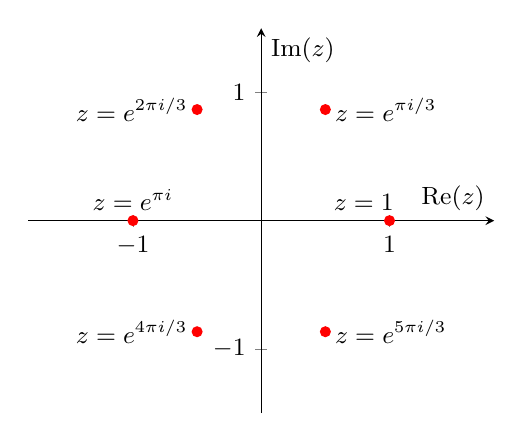
\begin{tikzpicture}
                \begin{axis}[
                    font=\small,
                    xmin=-1.5,
                    xmax=1.5,
                    ymin=-1.5,
                    ymax=1.5,
                    axis equal,
                    axis lines=middle,
                    xlabel=Re($z$),
                    ylabel=Im($z$),
                    ]
                    \fill [red] ({cos(0)},{(sin(0))}) circle (2pt);
                    \node [anchor=south] at ({cos(0) - 0.2},{(sin(0))}) {$z = 1$};

                    \fill [red] ({cos(1 * 360/6)},{(sin(1 * 360/6))}) circle (2pt);
                    \node [anchor=west] at ({cos(1 * 360/6)},{(sin(1 * 360/6))}) {$z = e^{\pi i/3}$};

                    \fill [red] ({cos(2 * 180/3)},{(sin(2 * 180/3))}) circle (2pt);
                    \node [anchor=east] at ({cos(2 * 180/3)},{(sin(2 * 180/3))}) {$z = e^{2\pi i/3}$};

                    \fill [red] ({cos(3 * 180/3)},{(sin(3 * 180/3))}) circle (2pt);
                    \node [anchor=south] at ({cos(3 * 180/3)},{(sin(3 * 180/3))}) {$z = e^{\pi i}$};

                    \fill [red] ({cos(4 * 180/3)},{(sin(4 * 180/3))}) circle (2pt);
                    \node [anchor=east] at ({cos(4 * 180/3)},{(sin(4 * 180/3))}) {$z = e^{4\pi i/3}$};

                    \fill [red] ({cos(5 * 180/3)},{(sin(5 * 180/3))}) circle (2pt);
                    \node [anchor=west] at ({cos(5 * 180/3)},{(sin(5 * 180/3))}) {$z = e^{5\pi i/3}$};
                \end{axis}
            \end{tikzpicture}
        \end{tabular}
        
    \end{center}
    \newpage
    De som van de n eenheidswortels is 0, omdat alle vectoren opgetelt elkaar opheffen. Wanneer $n$ even is, zoals bij $n = 6$, heffen alle getallen met een complex deel niet gelijk aan 0 elkaar op, en blijven alleen -1 en 1 over die elkaar vervolgens opheffen. Wanneer $n$ oneven is, is de som van alle complexe getallen -1, wat vervolgens de overgebleven 1 opheft.
    
    Voorbeelden:
    \begin{center}
        $n = 3$
    \end{center}
    \begin{center}
        \begin{tikzpicture}
            \begin{axis}[
                font=\small,
                xmin=-1.5,
                xmax=1.5,
                ymin=-1.5,
                ymax=1.5,
                axis equal,
                axis lines=middle,
                xlabel=Re($z$),
                ylabel=Im($z$),
                ]

                \fill [red] ({cos(0)},{(sin(0))}) circle (2pt);
                \node [anchor=south] at ({cos(0) - 0.2},{(sin(0))}) {$z = 1$};

                \fill [red] ({cos(1 * 360/3)},{(sin(1 * 360/3))}) circle (2pt);
                \node [anchor=east] at ({cos(1 * 360/3)},{(sin(1 * 360/3))}) {$z = e^{2\pi i/3}$};

                \fill [red] ({cos(2 * 360/3)},{(sin(2 * 360/3))}) circle (2pt);
                \node [anchor=east] at ({cos(2 * 360/3)},{(sin(2 * 360/3))}) {$z = e^{4\pi i/3}$};

                \draw[dashed, ->] (0,0) -- ({cos(2 * 360/3)},{(sin(2 * 360/3))});
                \draw[->] (0,0) -- ({cos(1 * 360/3)},{(sin(1 * 360/3))});
                \draw[->] ({cos(1 * 360/3)},{(sin(1 * 360/3))}) -- (-1,0);
            \end{axis}
        \end{tikzpicture}
    \end{center}
    \begin{center}
        \footnotesize We zien hier dat de som van de twee complexe getallen behalve 1, samen opgetelt -1 zijn. Dit heft op met de overgebleven eenheidswortel 1, en houden we 0 over.        
    \end{center}

    \begin{center}
        $n = 6$
    \end{center}
    \begin{center}
        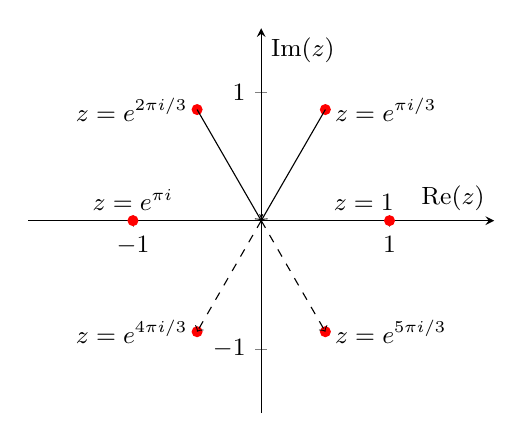
\begin{tikzpicture}
            \begin{axis}[
                font=\small,
                xmin=-1.5,
                xmax=1.5,
                ymin=-1.5,
                ymax=1.5,
                axis equal,
                axis lines=middle,
                xlabel=Re($z$),
                ylabel=Im($z$),
                ]
                \fill [red] ({cos(0)},{(sin(0))}) circle (2pt);
                \node [anchor=south] at ({cos(0) - 0.2},{(sin(0))}) {$z = 1$};

                \fill [red] ({cos(1 * 360/6)},{(sin(1 * 360/6))}) circle (2pt);
                \node [anchor=west] at ({cos(1 * 360/6)},{(sin(1 * 360/6))}) {$z = e^{\pi i/3}$};

                \fill [red] ({cos(2 * 180/3)},{(sin(2 * 180/3))}) circle (2pt);
                \node [anchor=east] at ({cos(2 * 180/3)},{(sin(2 * 180/3))}) {$z = e^{2\pi i/3}$};

                \fill [red] ({cos(3 * 180/3)},{(sin(3 * 180/3))}) circle (2pt);
                \node [anchor=south] at ({cos(3 * 180/3)},{(sin(3 * 180/3))}) {$z = e^{\pi i}$};

                \fill [red] ({cos(4 * 180/3)},{(sin(4 * 180/3))}) circle (2pt);
                \node [anchor=east] at ({cos(4 * 180/3)},{(sin(4 * 180/3))}) {$z = e^{4\pi i/3}$};

                \fill [red] ({cos(5 * 180/3)},{(sin(5 * 180/3))}) circle (2pt);
                \node [anchor=west] at ({cos(5 * 180/3)},{(sin(5 * 180/3))}) {$z = e^{5\pi i/3}$};

                \draw[dashed, ->] (0,0) -- ({cos(4 * 180/3)},{(sin(4 * 180/3))});
                \draw[dashed, ->] (0,0) -- ({cos(5 * 180/3)},{(sin(5 * 180/3))});

                \draw[->] ({cos(1 * 180/3)},{(sin(1 * 180/3))}) -- (0,0);
                \draw[->] ({cos(2 * 180/3)},{(sin(2 * 180/3))}) -- (0,0);
            \end{axis}
        \end{tikzpicture}
    \end{center}
    \begin{center}
        \footnotesize We zien hier dat de som van de complexe getallen die niet op de reële as liggen 0 is, en vervolgens -1 en 1 overblijven. Deze twee heffen elkaar op, en houden we 0 over.
    \end{center}
    \bigskip
    \item 
    De n-de eenheidswortels zijn $z = e^{\frac{2k\pi i}{n}}$ met $k \in \mathbb{N}$. Voor afleiding zie opdracht \ref{opdrachta}

    De n-de eenheidswortels zijn weer te geven in het complexe vlak als punten die gelijkmatig zijn verdeeld over de eenheidscirkel. Er zijn altijd n aantal eenheidswortels. De hoek tussen twee opeenvolgende eenheidswortels is altijd $\frac{2\pi}{n}$.

    \item 
    Neem $w = e^{\frac{2\pi i}{n}}$ de eenheidswortel met het kleinste positieve argument, dan zijn de overige eenheidswortels te schrijven als $w^k$ voor een $k \in \mathbb{N}$, want ${(e^{\frac{2\pi i}{n}})}^k = e^{\frac{2k\pi i}{n}}$ is de algemene vorm van de eenheidswortels.
    \newpage
    \item \label{opdrachtd}
    Te bewijzen: $1 + w + w^2 + \dots + w^{n - 1} = 0$.

    \begin{proof}
        $ $\newline
        Neem $S = 1 + w + w^2 + \dots + w^{n - 1}$. \newline
        Dan $S \cdot w = w + w^2 + \dots + w^n = S - 1 + w^n$. \newline
        Dan kunnen we schrijven $S\cdot w - S = -1 + w^n$. \newline
        Omdat $w^n = {(e^{\frac{2\pi i}{n}})}^n = e^{2\pi i} = 1$, $-1 + w^n = 0$. \newline
        Dus $s(w - 1) = 0$ geeft $S = 1 + w + w^2 + \dots + w^{n - 1} = 0$.
    \end{proof}

    \item 
    Elke term in de som $1 + w + w^2 + \dots + w^{n - 1}$ corrospondeerd exact met een eenheidswortel en alle eenheidswortels corrosponderen exact met een term in deze som. Bij \ref{opdrachtd} \!hebben we bewezen dat deze som gelijk is aan 0, dus de som van alle eenheidswortels is 0.
\end{enumerate}









\end{document}